\section*{Introduction}

\PARstart{T}{he} recent development of various methods of modulation
such as PCM and PPM which exchange bandwidth for signal-to-noise ratio
has intensified the interest in a general theory of communication.
A basis for such a theory is contained in the important papers of
Nyquist\footnote{Nyquist, H., ``Certain Factors Affecting Telegraph
Speed,'' {\it Bell System Technical Journal,} April 1924, p.~324; ``Certain
Topics in Telegraph Transmission Theory,'' {\it A.I.E.E. Trans.,} v.~47,
April 1928, p.~617.} and Hartley\footnote{Hartley, R. V. L., ``Transmission
of Information,'' {\it Bell System Technical Journal,} July 1928, p.~535.}
on this subject.  In the present paper we will extend the theory to include
a number of new factors, in particular the effect of noise in the channel,
and the savings possible due to the statistical structure of the original
message and due to the nature of the final destination of the information.

The fundamental problem of communication is that of reproducing at one
point either exactly or approximately a message selected at another point.
Frequently the messages have \emph{meaning}; that is they refer to or are
correlated according to some system with certain physical or conceptual
entities.  These semantic aspects of communication are irrelevant to the
engineering problem.  The significant aspect is that the actual message is
one \emph{selected from a set} of possible messages.  The system must be
designed to operate for each possible selection, not just the one which
will actually be chosen since this is unknown at the time of design.

If the number of messages in the set is finite then this number or any
monotonic function of this number can be regarded as a measure of the
information produced when one message is chosen from the set, all choices
being equally likely.  As was pointed out by Hartley the most natural
choice is the logarithmic function.  Although this definition must be
generalized considerably when we consider the influence of the statistics
of the message and when we have a continuous range of messages, we will in
all cases use an essentially logarithmic measure.

The logarithmic measure is more convenient for various reasons:
\begin{enumerate}
\item
\label{it:0.1}
It is practically more useful.  Parameters of engineering importance such as
time, bandwidth, number of relays, etc., tend to vary linearly with the
logarithm of the number of possibilities.  For example, adding one relay to
a group doubles the number of possible states of the relays.  It adds 1 to
the base~2 logarithm of this number.  Doubling the time roughly squares the
number of possible messages, or doubles the logarithm, etc.
\item
It is nearer to our intuitive feeling as to the proper measure.  This is
closely related to~(\ref{it:0.1}) since we intuitively measures entities by
linear comparison with common standards.  One feels, for example, that two
punched cards should have twice the capacity of one for information
storage, and two identical channels twice the capacity of one for
transmitting information.
\item
It is mathematically more suitable.  Many of the limiting operations are
simple in terms of the logarithm but would require clumsy restatement in
terms of the number of possibilities.
\end{enumerate}

The choice of a logarithmic base corresponds to the choice of a unit for
measuring information.  If the base~2 is used the resulting units may be
called binary digits, or more briefly \emph{bits,} a word suggested by
J.~W.~Tukey.  A device with two stable positions, such as a relay or a
flip-flop circuit, can store one bit of information.  $N$ such devices can
store $N$ bits, since the total number of possible states is $2^N$ and
$\log_2 2^N=N$.  If the base~10 is used the units may be called decimal
digits.  Since
\begin{align*}
\log_2 M&=\log_{10}M/\log_{10}2\\
	&=3.32\log_{10}M,
\end{align*}
a decimal digit is about $3\frac13$ bits.  A digit wheel on a desk
computing machine has ten stable positions and therefore has a storage
capacity of one decimal digit.  In analytical work where integration and
differentiation are involved the base $e$ is sometimes useful.  The
resulting units of information will be called natural units.  Change from
the base $a$ to base $b$ merely requires multiplication by $\log_b a$.

By a communication system we will mean a system of the type indicated
schematically in Fig.~\ref{fig:1}.  It consists of essentially five parts:
\begin{enumerate}
\item
An \emph{information source} which produces a message or sequence of
messages to be communicated to the receiving terminal.  The message may be
of various types: (a) A sequence of letters as in a telegraph of
teletype system; (b) A single function of time $f(t)$ as in radio or
telephony; (c) A function of time and other variables as in black and white
television --- here the message may be thought of as a function $f(x,y,t)$ of
two space coordinates and time, the light intensity at point $(x,y)$ and
time $t$ on a pickup tube plate; (d) Two or more functions of time, say
$f(t)$, $g(t)$, $h(t)$ --- this is the case in ``three-dimensional'' sound
transmission or if the system is intended to service several individual
channels in multiplex; (e) Several functions of several variables --- in
color television the message consists of three functions $f(x,y,t)$,
$g(x,y,t)$, $h(x,y,t)$ defined in a three-dimensional continuum --- we may
also think of these three functions as components of a vector field defined
in the region --- similarly, several black and white television sources would
produce ``messages'' consisting of a number of functions of three
variables; (f) Various combinations also occur, for example in television
with an associated audio channel.
\item
A \emph{transmitter} which operates on the message in some way to produce a
signal suitable for transmission over the channel.  In telephony this
operation consists merely of changing sound pressure into a proportional
electrical current.  In telegraphy we have an encoding operation which
produces a sequence of dots, dashes and spaces on the channel corresponding
to the message.  In a multiplex PCM system the different speech functions
\begin{figure}
\centerline{\begin{picture}(0,0)%
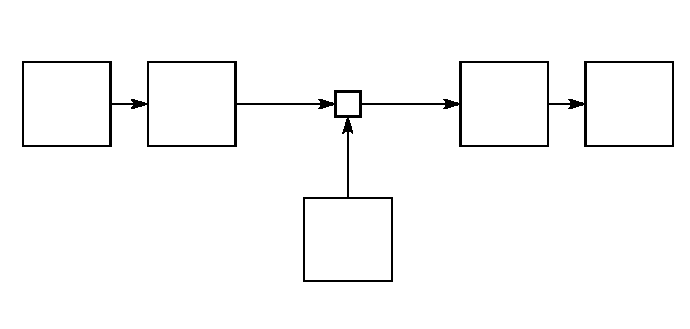
\epsfig{file=fig1.ps}%
\end{picture}%
\begin{small}%
\setlength{\unitlength}{1bp}%
\begin{picture}(315,142)
\put(24,134){\makebox(0,0){\sc information}}
\put(24,126){\makebox(0,0){\sc source}}
\put(52,73){\makebox(0,0){\sc message}}
\put(84,126){\makebox(0,0){\sc transmitter}}
\put(129,94){\makebox(0,0){\sc signal}}
\put(189,94){\makebox(0,0){\sc received}}
\put(189,87){\makebox(0,0){\sc signal}}
\put(234,126){\makebox(0,0){\sc receiver}}
\put(264,73){\makebox(0,0){\sc message}}
\put(294,126){\makebox(0,0){\sc destination}}
\put(161,8){\makebox(0,0){\sc noise}}
\put(161,1){\makebox(0,0){\sc source}}
\end{picture}%
\end{small}%
\endinput
}
\caption{Schematic diagram of a general communication system.}
\label{fig:1}
\end{figure}
must be sampled, compressed, quantized and encoded, and finally interleaved
properly to construct the signal.  Vocoder systems, television and
frequency modulation are other examples of complex operations applied to
the message to obtain the signal.
\item
The \emph{channel} is merely the medium used to transmit the signal from
transmitter to receiver.  It may be a pair of wires, a coaxial cable, a
band of radio frequencies, a beam of light, etc.

\item
The \emph{receiver} ordinarily performs the inverse operation of that done
by the transmitter, reconstructing the message from the signal.
\item
The \emph{destination} is the person (or thing) for whom the message is
intended.
\end{enumerate}

We wish to consider certain general problems involving communication
systems.  To do this it is first necessary to represent the various elements
involved as mathematical entities, suitably idealized from their physical
counterparts.  We may roughly classify communication systems into three main
categories: discrete, continuous and mixed.  By a discrete system we will
mean one in which both the message and the signal are a sequence of
discrete symbols.  A typical case is telegraphy where the message is a
sequence of letters and the signal a sequence of dots, dashes and
spaces.  A continuous system is one in which the message and signal are
both treated as continuous functions, e.g., radio or television.  A mixed
system is one in which both discrete and continuous variables appear, e.g.,
PCM transmission of speech.

We first consider the discrete case.  This case has applications not only
in communication theory, but also in the theory of computing machines, the
design of telephone exchanges and other fields.  In addition the discrete
case forms a foundation for the continuous and mixed cases which will be
treated in the second half of the paper.

